\definecolor{basiccnn}{HTML}{5B8DB8}
\definecolor{resnetcol}{HTML}{2E6DA4}
\definecolor{resnetse}{HTML}{1B4F72}
\definecolor{googlenet}{HTML}{7FB3D3}
\definecolor{effnet}{HTML}{1A5276}
\definecolor{cct}{HTML}{85C1E9}
\definecolor{ir50col}{HTML}{154360}
\definecolor{mamba}{HTML}{A9CCE3}
\definecolor{gridcolor}{HTML}{CCCCCC}

\begin{figure*}
\centering
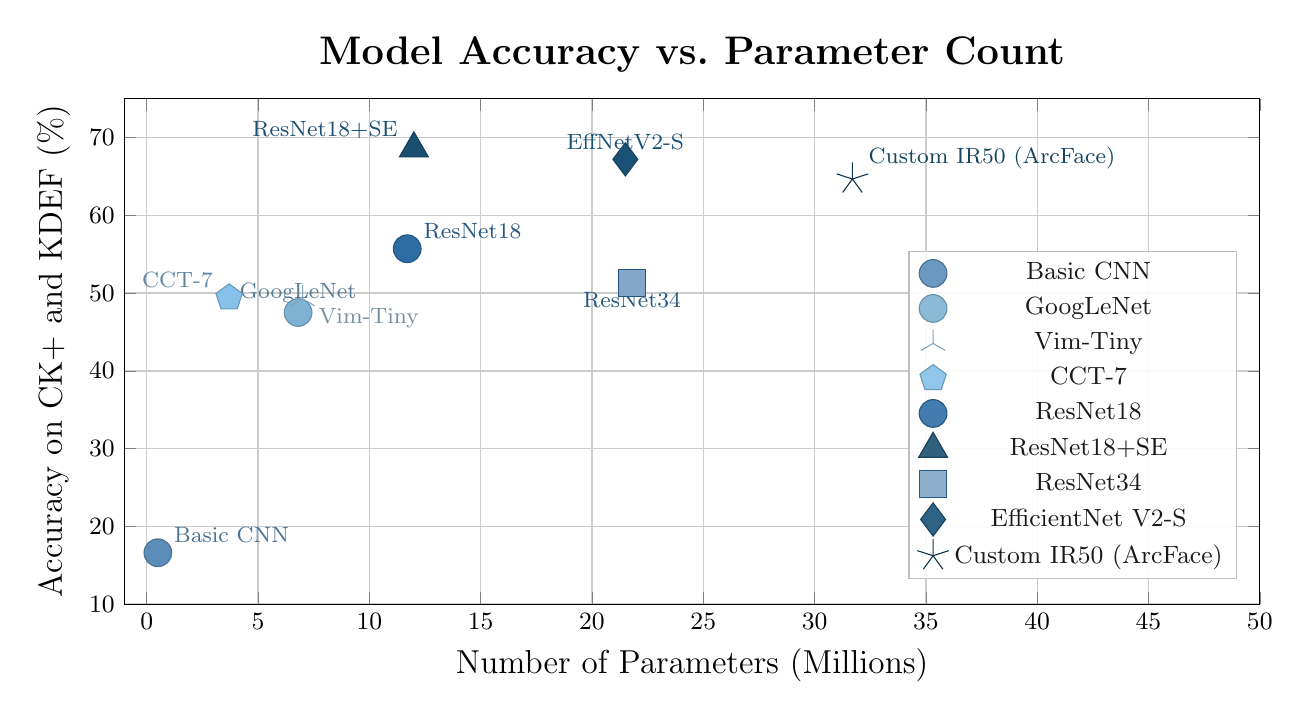
\begin{tikzpicture}
\begin{axis}[
    width=16cm,
    height=8cm,
    xlabel={\large Number of Parameters (Millions)},
    ylabel={\large Accuracy on CK+ and KDEF (\%)},
    title={\Large \textbf{Model Accuracy vs.\ Parameter Count}},
    xmin=-1, xmax=50,
    ymin=10, ymax=75,
    xtick={0,5,10,15,20,25,30,35,40,45,50},
    ytick={10,20,30,40,50,60,70},
    grid=both,
    grid style={line width=0.3pt, draw=gridcolor!60},
    major grid style={line width=0.5pt, draw=gridcolor},
    legend style={
        at={(0.98,0.05)}, anchor=south east,
        font=\small, fill=white, fill opacity=0.9,
        draw=gray!50, row sep=1pt,
    },
    tick label style={font=\small},
    clip=false,
]

\addplot[only marks, mark=*, mark size=5pt,
    draw=basiccnn!80!black, fill=basiccnn]
    coordinates {(0.5, 16.6)};
\addlegendentry{Basic CNN}
\node[anchor=south west, font=\footnotesize, text=basiccnn!80!black]
    at (axis cs:0.5,16.6) {\;Basic CNN};

\addplot[only marks, mark=*, mark size=5pt,
    draw=googlenet!80!black, fill=googlenet]
    coordinates {(6.8, 47.5)};
\addlegendentry{GoogLeNet}
\node[anchor=south, font=\footnotesize, text=googlenet!70!black]
    at (axis cs:6.8, 47.5) {GoogLeNet};

\addplot[only marks, mark=Mercedes star, mark size=5pt,
    draw=mamba!80!black, fill=mamba]
    coordinates {(7.0, 49.26)};
\addlegendentry{Vim-Tiny}
\node[anchor=north west, font=\footnotesize, text=mamba!70!black]
    at (axis cs:7.0, 49.26) {\;Vim-Tiny};

\addplot[only marks, mark=pentagon*, mark size=5pt,
    draw=cct!80!black, fill=cct]
    coordinates {(3.7, 49.4)};
\addlegendentry{CCT-7}
\node[anchor=south east, font=\footnotesize, text=cct!70!black]
    at (axis cs:3.7, 49.4) {CCT-7\;};

\addplot[only marks, mark=*, mark size=5pt,
    draw=resnetcol!80!black, fill=resnetcol]
    coordinates {(11.7, 55.7)};
\addlegendentry{ResNet18}
\node[anchor=south west, font=\footnotesize, text=resnetcol!80!black]
    at (axis cs:11.7, 55.7) {\;ResNet18};

\addplot[only marks, mark=triangle*, mark size=6pt,
    draw=resnetse!80!black, fill=resnetse]
    coordinates {(12.0, 68.6)};
\addlegendentry{ResNet18+SE}
\node[anchor=south east, font=\footnotesize, text=resnetse]
    at (axis cs:12.0, 68.6) {ResNet18+SE\;};

\addplot[only marks, mark=square*, mark size=5pt,
    draw=resnetcol!80!black, fill=resnetcol!60]
    coordinates {(21.8, 51.3)};
\addlegendentry{ResNet34}
\node[anchor=north, font=\footnotesize, text=resnetcol!80!black]
    at (axis cs:21.8, 51.3) {ResNet34};

\addplot[only marks, mark=diamond*, mark size=6pt,
    draw=effnet!80!black, fill=effnet]
    coordinates {(21.5, 67.2)};
\addlegendentry{EfficientNet V2-S}
\node[anchor=south, font=\footnotesize, text=effnet]
    at (axis cs:21.5, 67.2) {EffNetV2-S};

\addplot[only marks, mark=star, mark size=6pt,
    draw=ir50col!80!black, fill=ir50col]
    coordinates {(31.7, 64.67)};
\addlegendentry{Custom IR50 (ArcFace)}
\node[anchor=south west, font=\footnotesize, text=ir50col]
    at (axis cs:31.7, 64.67) {\;Custom IR50 (ArcFace)};

\end{axis}
\end{tikzpicture}
\caption{Model Accuracy vs. Parameter Count evaluated on the CK+ and KDEF datasets.}
\label{fig:accuracy_vs_params}
\end{figure*}

\section{Conclusion}

This project successfully developed a comprehensive emotion classification system for facial expressions. We implemented a complete pipeline from raw image data through preprocessing to model training and evaluation, utilizing state-of-the-art deep learning techniques.

\subsection{Key Contributions}

\begin{enumerate}
    \item \textbf{Robust Preprocessing Pipeline}: Developed comprehensive preprocessing procedures including face detection, alignment, deduplication, and quality filtering that significantly improved dataset quality and model robustness.
    
    \item \textbf{Attention-Enhanced Architecture}: Integrated Squeeze-and-Excitation blocks into ResNet-18, demonstrating consistent performance improvements over baseline models.
    
    \item \textbf{Class-Balanced Training}: Employed focal loss to address class imbalance, resulting in more balanced performance across emotion categories.
    
    \item \textbf{Multi-Dataset Evaluation}: Comprehensive evaluation across multiple emotion datasets demonstrated model generalization capabilities and robustness across domain shifts.
    
    \item \textbf{Model Interpretability}: Applied Grad-CAM visualization to validate that the model learns emotion-specific facial features, providing insight into the decision-making process.
\end{enumerate}

\subsection{Limitations and Future Work}

While our system achieves competitive performance, several limitations and opportunities for future work exist:

\subsubsection{Limitations}

\begin{itemize}
    \item Performance degradation on low-quality images and extreme face angles
    \item Difficulty distinguishing between similar emotions (fear/surprise, anger/disgust)
    \item Limited robustness to occlusions and non-frontal faces
    \item Dependency on extensive preprocessing and high-quality face detection
\end{itemize}

\subsubsection{Future Directions}

\begin{itemize}
    \item Exploration of transformer-based architectures (Vision Transformers, Compact Transformers) for potentially improved performance
    \item Integration of temporal information for video-based emotion recognition
    \item Development of robust multi-task learning approaches combining emotion, age, gender, and identity recognition
    \item Investigation of domain adaptation techniques to improve cross-dataset generalization
    \item Incorporation of action unit detection for finer-grained emotion understanding
    \item Real-time deployment optimization for mobile and edge devices
\end{itemize}

\subsection{Final Remarks}

The facial emotion classification system presented in this report demonstrates the effectiveness of combining careful data preprocessing, attention mechanisms, and appropriate loss functions for emotion recognition tasks. The model's interpretability through Grad-CAM analysis confirms that it learns meaningful emotional representations. Future work should focus on improving robustness to challenging conditions and exploring more advanced architecture designs, particularly with emerging transformer-based models. The comprehensive multi-dataset evaluation framework established in this project provides a solid foundation for continued research in this important area of computer vision.
